\documentclass[a4paper]{article}
\usepackage{amsmath,amssymb,float,geometry,graphicx,minted,pgfplots,tikz,xcolor}
\definecolor{ntype}{RGB}{162,192,217}
\definecolor{depletionregion}{RGB}{212,212,212}
\definecolor{ptype}{RGB}{152,230,152}
\definecolor{efield}{RGB}{169,171,174}
\geometry{left=3.5cm,right=3.5cm,top=3.3cm,bottom=3.3cm}
\renewcommand\thesection{\arabic{section}}
\usetikzlibrary {backgrounds}
% \usetikzlibrary {datavisualization}
% \graphicspath{{svg/}}
% \newcommand{\executeiffilenewer}[3]{%
  % \ifnum\pdfstrcmp{\pdffilemoddate{#1}}%
  % {\pdffilemoddate{#2}}>0%
  % {\immediate\write18{#3}}\fi%
% }
% \newcommand{\includesvg}[2]{%
% \executeiffilenewer{svg/#2.svg}{svg/#2.pdf}%
% {inkscape -D --export-filename=svg/#2.pdf svg/#2.svg}%
% \includegraphics[width=#1]{#2.pdf}%
% }
\begin{document}
\begin{center}
\huge
\textbf{VE320\\Intro to Semiconductor Devices\\}
\Large
\vspace{30pt}
\uppercase{Homework 6}\\
\vspace{5pt}\today\\
\vspace{5pt}
Yihua Liu 518021910998
\vspace{5pt}
\rule[-10pt]{.97\linewidth}{0.05em}
\end{center}
% \begin{figure}[H]
    % \centering
    % \includesvg{1\columnwidth}{1}
    % \caption{}
% \end{figure}
1. (a) Sketch of the energy-band diagram.

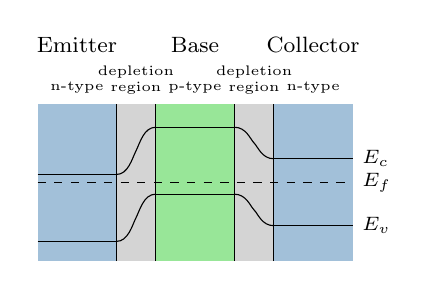
\begin{tikzpicture}
    \draw (0,1.1) -- (1,1.1);
    \draw (1,1.1) .. controls (1.15,1.1) and (1.2,1.3) .. (1.25,1.4);
    \draw (1.25,1.4) .. controls (1.3,1.5) and (1.35,1.7) .. (1.5,1.7);
    \draw (1.5,1.7) -- (2.5,1.7);
    \draw (2.5,1.7) .. controls (2.65,1.7) and (2.7,1.55) .. (2.75,1.5);
    \draw (2.75,1.5) .. controls (2.8,1.45) and (2.85,1.3) .. (3,1.3);
    \draw (3,1.3) -- (4,1.3) node[right] {\scriptsize $E_c$};
    \draw (0,0.25) -- (1,0.25);
    \draw (1,0.25) .. controls (1.15,0.25) and (1.2,0.45) .. (1.25,0.55);
    \draw (1.25,0.55) .. controls (1.3,0.65) and (1.35,0.85) .. (1.5,0.85);
    \draw (1.5,0.85) -- (2.5,0.85);
    \draw (2.5,0.85) .. controls (2.65,0.85) and (2.7,0.7) .. (2.75,0.65);
    \draw (2.75,0.65) .. controls (2.8,0.6) and (2.85,0.45) .. (3,0.45);
    \draw (3,0.45) -- (4,0.45) node[right] {\scriptsize $E_v$};
    \draw (1,0) -- (1,2);
    \draw (1.5,0) -- (1.5,2);
    \draw (2.5,0) -- (2.5,2);
    \draw (3,0) -- (3,2);
    \draw [dashed] (0,1) -- (4,1) node[right] {\scriptsize $E_f$};
    \node at (0.5,2.2) {\tiny n-type};
    \node at (1.25,2.3) {\tiny
        \begin{tabular}{c}
            depletion\\
            region\\
        \end{tabular}
    };
    \node at (2,2.2) {\tiny p-type};
    \node at (2.75,2.3) {\tiny
        \begin{tabular}{c}
            depletion\\
            region\\
        \end{tabular}
    };
    \node at (3.5,2.2) {\tiny n-type};
    \node at (0.5,2.75) {\footnotesize Emitter};
    \node at (2,2.75) {\footnotesize Base};
    \node at (3.5,2.75) {\footnotesize Collector};
    \begin{scope}[on background layer]
        \fill[ntype] (0,0) rectangle (1,2);
        \fill[depletionregion] (1,0) rectangle (1.5,2);
        \fill[ptype] (1.5,0) rectangle (2.5,2);
        \fill[depletionregion] (2.5,0) rectangle (3,2);
        \fill[ntype] (3,0) rectangle (4,2);
    \end{scope}
\end{tikzpicture}

(b) Sketch of the electric field through the device.

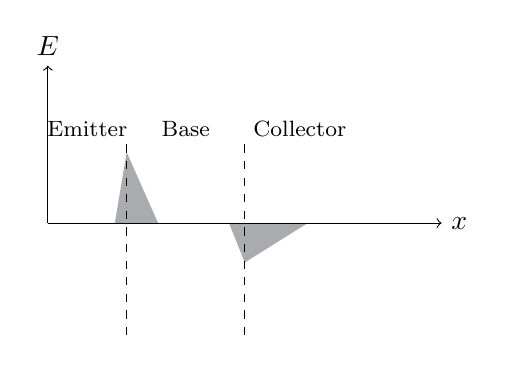
\begin{tikzpicture} 
    \draw[->] (0,0) -- (5,0) node[right] {$x$};
    \draw[->] (0,0) -- (0,2) node[above] {$E$};
    \draw [dashed] (1,1) -- (1,-1.5);
    \draw [dashed] (2.5,1) -- (2.5,-1.5);
    \node at (0.5,1.2) {\footnotesize Emitter};
    \node at (1.75,1.2) {\footnotesize Base};
    \node at (3.2,1.2) {\footnotesize Collector};
    \begin{pgfonlayer}{background}
        \fill[efield] (0.85,0) -- (1,0.9) -- (1.4,0) -- cycle;
        \fill[efield] (2.3,0) -- (2.5,-0.5) -- (3.3,0) -- cycle;
    \end{pgfonlayer}
\end{tikzpicture}

(c) Sketch of the energy-band diagram in the forward-active region.

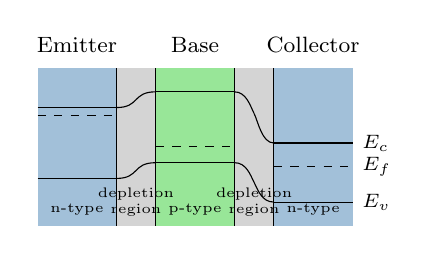
\begin{tikzpicture}
    \draw (0,1.5) -- (1,1.5);
    \draw (1,1.5) .. controls (1.15,1.5) and (1.2,1.55) .. (1.25,1.6);
    \draw (1.25,1.6) .. controls (1.3,1.65) and (1.35,1.7) .. (1.5,1.7);
    \draw (1.5,1.7) -- (2.5,1.7);
    \draw (2.5,1.7) .. controls (2.65,1.7) and (2.7,1.525) .. (2.75,1.425);
    \draw (2.75,1.425) .. controls (2.8,1.325) and (2.85,1.05) .. (3,1.05);
    \draw (3,1.05) -- (4,1.05) node[right] {\scriptsize $E_c$};
    \draw (0,0.6) -- (1,0.6);
    \draw (1,0.6) .. controls (1.15,0.6) and (1.2,0.65) .. (1.25,0.7);
    \draw (1.25,0.7) .. controls (1.3,0.75) and (1.35,0.8) .. (1.5,0.8);
    \draw (1.5,0.8) -- (2.5,0.8);
    \draw (2.5,0.8) .. controls (2.65,0.8) and (2.7,0.65) .. (2.75,0.55);
    \draw (2.75,0.55) .. controls (2.8,0.45) and (2.85,0.3) .. (3,0.3);
    \draw (3,0.3) -- (4,0.3) node[right] {\scriptsize $E_v$};
    \draw (1,0) -- (1,2);
    \draw (1.5,0) -- (1.5,2);
    \draw (2.5,0) -- (2.5,2);
    \draw (3,0) -- (3,2);
    \draw [dashed] (0,1.4) -- (1,1.4);
    \draw [dashed] (1.5,1) -- (2.5,1);
    \draw [dashed] (3,0.75) -- (4,0.75) node[right] {\scriptsize $E_f$};
    \node at (0.5,0.2) {\tiny n-type};
    \node at (1.25,0.3) {\tiny
        \begin{tabular}{c}
            depletion\\
            region\\
        \end{tabular}
    };
    \node at (2,0.2) {\tiny p-type};
    \node at (2.75,0.3) {\tiny
        \begin{tabular}{c}
            depletion\\
            region\\
        \end{tabular}
    };
    \node at (3.5,0.2) {\tiny n-type};
    \node at (0.5,2.3) {\footnotesize Emitter};
    \node at (2,2.3) {\footnotesize Base};
    \node at (3.5,2.3) {\footnotesize Collector};
    \begin{scope}[on background layer]
        \fill[ntype] (0,0) rectangle (1,2);
        \fill[depletionregion] (1,0) rectangle (1.5,2);
        \fill[ptype] (1.5,0) rectangle (2.5,2);
        \fill[depletionregion] (2.5,0) rectangle (3,2);
        \fill[ntype] (3,0) rectangle (4,2);
    \end{scope}
\end{tikzpicture}

Sketch of the electric field through the device in the forward-active region.

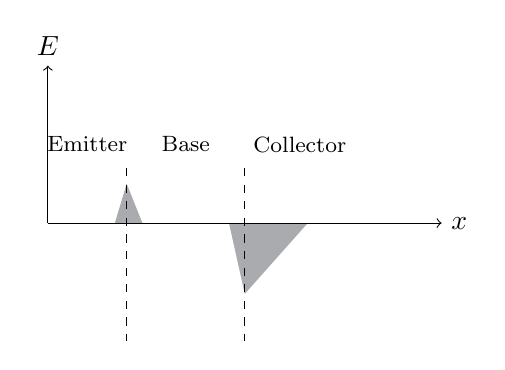
\begin{tikzpicture} 
    \draw[->] (0,0) -- (5,0) node[right] {$x$};
    \draw[->] (0,0) -- (0,2) node[above] {$E$};
    \draw [dashed] (1,0.7) -- (1,-1.5);
    \draw [dashed] (2.5,0.7) -- (2.5,-1.5);
    \node at (0.5,1) {\footnotesize Emitter};
    \node at (1.75,1) {\footnotesize Base};
    \node at (3.2,1) {\footnotesize Collector};
    \begin{pgfonlayer}{background}
        \fill[efield] (0.85,0) -- (1,0.5) -- (1.2,0) -- cycle;
        \fill[efield] (2.3,0) -- (2.5,-0.9) -- (3.3,0) -- cycle;
    \end{pgfonlayer}
\end{tikzpicture}

2. (a) The thermal-equilibrium values
$$p_{E0}=\frac{n_i^2}{N_E}=\frac{(1.5\times10^{10})^2}{8\times10^{17}}=281.25\ \mathrm{cm^{-3}}.$$
$$n_{B0}=\frac{n_i^2}{N_B}=\frac{(1.5\times10^{10})^2}{10^{16}}=2.25\times10^4\ \mathrm{cm^{-3}}.$$
$$p_{C0}=\frac{n_i^2}{N_C}=\frac{(1.5\times10^{10})^2}{10^{15}}=2.25\times10^5\ \mathrm{cm^{-3}}.$$

(b) The value of $n_B$ at $x=0$ for $V_{BE}=0.64$ V
$$n_B(0)=n_{B0}\bigg[\exp{\bigg(\frac{eV_{BE}}{kT}\bigg)}-1\bigg]=1.270\times10^{15}\ \mathrm{cm^{-3}}.$$
The value of $p_E$ at $x'=0$ for $V_{BE}=0.64$ V
$$p_E(0)=p_{E0}\bigg[\exp{\bigg(\frac{eV_{BE}}{kT}\bigg)}-1\bigg]=1.587\times10^{13}\ \mathrm{cm^{-3}}.$$

(c)
\begin{figure}[H]
    \centering
    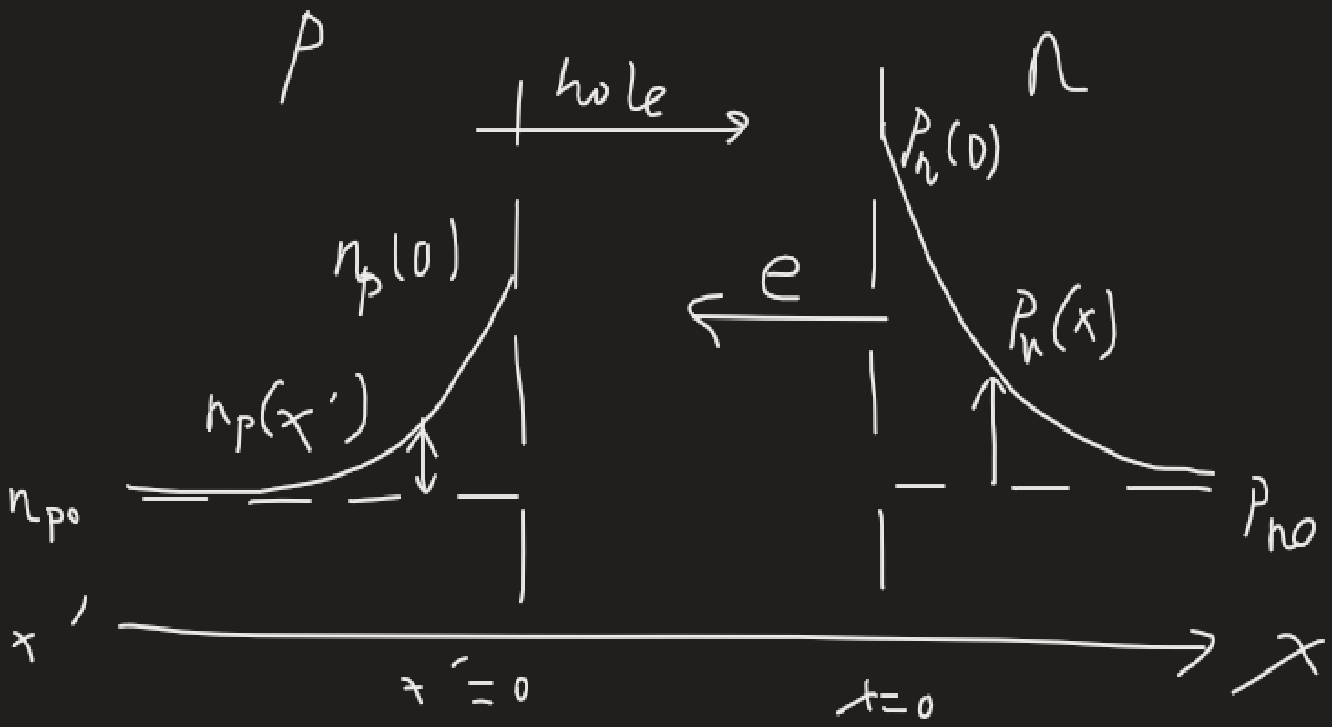
\includegraphics[width=1\textwidth]{0.png}
    \caption{The minority carrier concentrations through the device.}
\end{figure}
3. (a)
$$\gamma=\frac{I_{nE}}{I_{nE}+I_{pE}}=\frac{500}{500+3.5}=0.9930.$$
$$\alpha_T=\frac{I_{nC}}{I_{nE}}=\frac{0.495}{0.5}=0.99.$$
$$\delta=\frac{I_{nE}+I_{pE}}{I_{nE}+I_R+I_{pE}}=\frac{500+3.5}{500+5+3.5}=0.9902.$$
$$\alpha=\frac{I_{nC}}{I_{nE}+I_R+I_{pE}}=\frac{495}{500+5+3.5}=0.9735.$$
$$\beta=\frac{\alpha}{1-\alpha}=36.67.$$

(b) Given $\beta=120$,
$$\alpha=\frac{\beta}{1+\beta}=0.9917$$
Solving the equation $\gamma=\alpha_T=\delta$, we have
$$\frac{I_{nE}}{I_{nC}}=0.546.$$
Therefore,
$$I_{nC}=9.16\times10^{-4}\ \mathrm{A}.$$
$$I_{pE}=2.43\times10^{-4}\ \mathrm{A}.$$
$$I_R=1.49\times10^{-4}\ \mathrm{A}.$$

4. Substituting $\frac{n_i^2}{N_E}$ for $p_{E0}$, $\frac{n_i^2}{N_B}$ for $n_{E0}$, $N_E=100N_B$, $D_E=D_B$, $L_B=L_E$, $x_B=0.1L_B$, the emitter injection efficiency $\gamma$ is
$$\gamma=\frac{1}{1+\dfrac{p_{E0}D_EL_B}{n_{B0}D_BL_E}\cdot\dfrac{\tanh{(x_B/L_B)}}{\tanh{(x_E/L_E)}}}=\frac{1}{1+\dfrac{0.01\tanh{(0.1)}}{\tanh{(x_E/L_E)}}}.$$
The graph of the emitter injection efficiency for $0.01L_E\leq x_E\leq10L_E$ is
\begin{figure}[H]
    \centering
    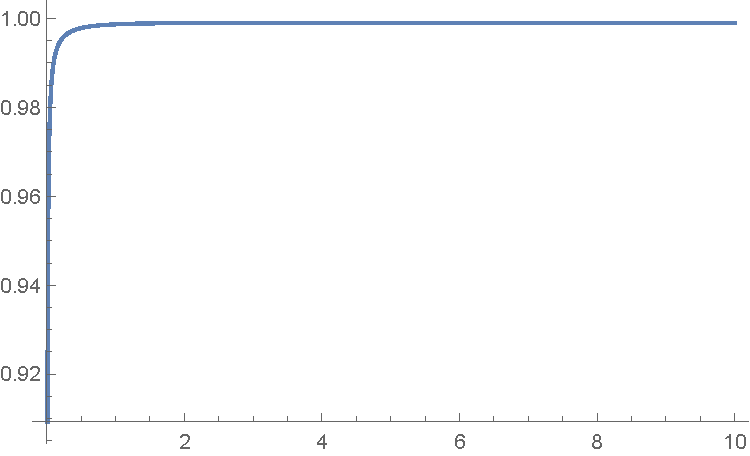
\includegraphics[width=1\textwidth]{1.eps}
    \caption{The graph of the emitter injection efficiency for $0.01L_E\leq x_E\leq10L_E$.}
\end{figure}
From these results, as the emitter width increases, the emitter injection efficiency increases to a constant, and the common emitter current gain increases.

5. (a) (i) The output resistance
$$r_o=\frac{V_{CE}+V_A}{I_C}=\frac{2+120}{1.2\times10^{-3}}=1.017\times10^5\ \Omega.$$
(ii) The output conductance
$$g_o=\frac{I_C}{V_{CE}+V_A}=9.836\times10^{-6}\ \Omega^{-1}.$$
(iii) The collector current
$$I_C=\frac{V_{CE}+V_A}{r_o}=1.220\times10^{-3}\ \mathrm{A}.$$

(b) (i) The output resistance
$$r_o=\frac{V_{CE}+V_A}{I_C}=\frac{2+160}{0.25\times10^{-3}}=6.48\times10^5\ \Omega.$$
(ii) The output conductance
$$g_o=\frac{I_C}{V_{CE}+V_A}=1.543\times10^{-6}\ \Omega^{-1}.$$
(iii) The collector current
$$I_C=\frac{V_{CE}+V_A}{r_o}=2.531\times10^{-4}\ \mathrm{A}.$$

6. (a) (i) Given $x_{BO}\ll L_B$, the excess minority carrier electron concentration in the base can be approximated by
$$\delta n_B(x)\cong\frac{n_{BO}}{x_B}\bigg\{\bigg[\exp{\bigg(\frac{V_{BE}}{V_t}\bigg)}-1\bigg](x_B-x)-x\bigg\}$$
The collector current is
$$|J_C|=eD_B\frac{d[\delta n_B(x)]}{dx}\cong\frac{eD_Bn_{BO}}{x_B}\exp{\bigg(\frac{V_{BE}}{V_t}\bigg)}$$
$$V_{bi}=\frac{kT}{e}\ln{\bigg(\frac{N_BN_C}{n_i^2}\bigg)}$$
$$x_{dB}=\sqrt{\frac{2\epsilon_s(V_{bi}+V_{BC})}{e}\cdot\frac{N_C}{N_B}\cdot\frac{1}{N_C+N_B}}$$
$$n_{BO}=\frac{n_i^2}{N_B}=1.125\times10^4\ \mathrm{cm^{-3}}$$
$$x_B=x_{BO}-x_{dB}$$
Solving the equations, the electron diffusion current density is
$$J_C=54.71\ \mathrm{A/cm^2}.$$
(ii) The electron diffusion current density is
$$J_C=59.97\ \mathrm{A/cm^2}.$$
(iii) The electron diffusion current density is
$$J_C=64.87\ \mathrm{A/cm^2}.$$

(b) We can estimate the Early voltage by
$$\frac{\Delta J_C}{\Delta V_{CE}}=\frac{J_C}{V_{CE}+V_A},$$
where $\Delta J_C$ is the difference between $J_C$ when $V_{CB}=4$ V and 12 V, $J_C$ is the electron diffusion current density when $V_{CB}=4$ V, $\Delta V_{CE}=12-4=8$ V. Solving the equation, the Early voltage is
$$V_A=50.11\ \mathrm{V}.$$

7. (a) From the results of 6(a), we have
$$V_{bi}=\frac{kT}{e}\ln{\bigg(\frac{N_BN_C}{n_i^2}\bigg)}$$
$$x_{dB}=\sqrt{\frac{2\epsilon_s(V_{bi}+V_{BC})}{e}\cdot\frac{N_C}{N_B}\cdot\frac{1}{N_C+N_B}}$$
Solving the equations, when $V_{BC}=1$ V,
$$x_{dB1}=1.386\times10^{-7}\ \mathrm{m},$$
when $V_{BC}=5$ V,
$$x_{dB1}=2.574\times10^{-7}\ \mathrm{m}.$$
The change in neutral base width as $V_{BC}$ changes from 1 to 5 V is
$$\Delta x_B=x_{B1}-x_{B2}=x_{B1}-x_{dB2}=1.188\times10^{-7}\ \mathrm{m}.$$

(b) The collector current is
$$I_C=\frac{eD_Bp_{BO}A_{BE}}{x_B}\exp{\bigg(\frac{eV_{EB}}{kT}\bigg)},$$
where
$$p_{BO}=\frac{n_i^2}{N_B}=2.25\times10^4\ \mathrm{cm^{-3}}.$$
Thus, when $V_{BC}=1$ V,
$$I_{C1}=2.028\times10^{-3}\ \mathrm{A},$$
when $V_{BC}=5$ V,
$$I_{C2}=2.573\times10^{-3}\ \mathrm{A}.$$
Thus, the corresponding change in collector current is
$$\Delta I_C=I_{C2}-I_{C1}=5.442\times10^{-4}\ \mathrm{A}.$$

(c) We can estimate the Early voltage by
$$\frac{\Delta I_C}{\Delta V_{BC}}=\frac{I_C}{V_{EC}+V_A},$$
where $I_C=I_{C1}$ is the collector current when $V_{BC}=5$ V, $\Delta V_{BC}=5-1=4\ \mathrm{V}$. Solving the equation, the Early voltage is
$$V_A=13.28\ \mathrm{V}.$$

(d) The output resistance is
$$r_o=\frac{V_{CE}+V_A}{I_C}=7.350\times10^3\ \Omega.$$
\end{document}